% Schematic for the metabolic flux feasibility example
% (CHEME-153-M2-MetabolicFluxFeasibility-MWA-Watch-Demo.ipynb)
%
% Bipartite structure: 5 reactions (fluxes/variables) draw on 3 enzymes (capacity constraints).
%   enzyme usage A[k,i] (rows = enzymes E1..E3, cols = reactions R1..R5):
%       E1: [1 0 2 0 1]   capacity b1 = 8
%       E2: [0 1 1 1 0]   capacity b2 = 5
%       E3: [1 1 0 0 2]   capacity b3 = 7
%   total flux budget sum(x) = tau = 10;  feasibility: find x in the simplex with A x <= b.
%
% Build:  pdflatex metabolic-flux.tex
\documentclass[border=10pt]{standalone}
\usepackage{amsmath}
\usepackage{tikz}
\usetikzlibrary{arrows.meta, positioning, calc, decorations.pathreplacing, backgrounds}

\begin{document}
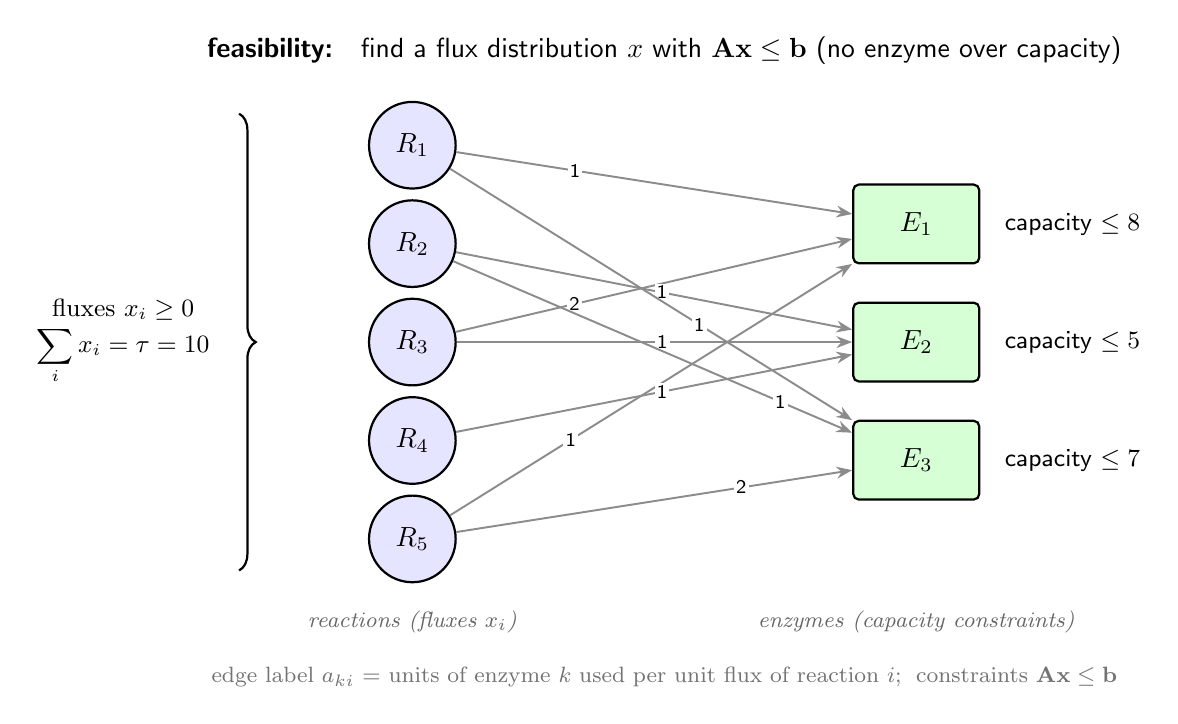
\begin{tikzpicture}[
    >={Stealth[length=2.4mm]},
    font=\sffamily,
    rxn/.style  = {circle, draw=black, line width=0.8pt, minimum size=11mm, inner sep=0pt, fill=blue!10},
    enz/.style  = {rounded corners=2pt, draw=black, line width=0.8pt,
                   minimum width=16mm, minimum height=10mm, fill=green!16},
    con/.style  = {-{Stealth[length=2.0mm]}, draw=black!45, line width=0.7pt},
    alab/.style = {font=\scriptsize\sffamily, fill=white, inner sep=0.8pt},
    ctag/.style = {font=\small\sffamily, anchor=west}
  ]

  % --- reactions (left column) ---
  \node[rxn] (R1) at (0,5.0) {$R_1$};
  \node[rxn] (R2) at (0,3.75){$R_2$};
  \node[rxn] (R3) at (0,2.5) {$R_3$};
  \node[rxn] (R4) at (0,1.25){$R_4$};
  \node[rxn] (R5) at (0,0.0) {$R_5$};

  % --- enzymes (right column) ---
  \node[enz] (E1) at (6.4,4.0) {$E_1$};
  \node[enz] (E2) at (6.4,2.5) {$E_2$};
  \node[enz] (E3) at (6.4,1.0) {$E_3$};

  % --- usage edges  R_i --a_{ki}--> E_k  (labels staggered by enzyme) ---
  \draw[con] (R1) -- node[alab,pos=0.30]{1} (E1);
  \draw[con] (R3) -- node[alab,pos=0.30]{2} (E1);
  \draw[con] (R5) -- node[alab,pos=0.30]{1} (E1);

  \draw[con] (R2) -- node[alab,pos=0.52]{1} (E2);
  \draw[con] (R3) -- node[alab,pos=0.52]{1} (E2);
  \draw[con] (R4) -- node[alab,pos=0.52]{1} (E2);

  \draw[con] (R1) -- node[alab,pos=0.62]{1} (E3);
  \draw[con] (R2) -- node[alab,pos=0.82]{1} (E3);
  \draw[con] (R5) -- node[alab,pos=0.72]{2} (E3);

  % --- capacity tags (right of each enzyme) ---
  \node[ctag] at (7.4,4.0) {capacity $\le 8$};
  \node[ctag] at (7.4,2.5) {capacity $\le 5$};
  \node[ctag] at (7.4,1.0) {capacity $\le 7$};

  % --- flux budget brace (far left) ---
  \draw[decorate, decoration={brace, amplitude=6pt}, line width=0.8pt]
       (-2.2,5.4) -- (-2.2,-0.4)
       node[midway, left=7pt, align=center, font=\small]
       {fluxes $x_i \ge 0$\\[2pt] $\displaystyle\sum_{i} x_i=\tau=10$};

  % --- feasibility framing (top) ---
  \node[align=center, font=\sffamily] at (3.2,6.2)
       {\textbf{feasibility:}\quad find a flux distribution $x$ with $\mathbf{A}\mathbf{x}\le\mathbf{b}$ (no enzyme over capacity)};

  % --- column captions + edge-label key (bottom) ---
  \node[font=\footnotesize\itshape, black!60] at (0,-1.05) {reactions (fluxes $x_i$)};
  \node[font=\footnotesize\itshape, black!60] at (6.4,-1.05) {enzymes (capacity constraints)};
  \node[font=\footnotesize, black!55, align=center] at (3.2,-1.75)
       {edge label $a_{ki}$ = units of enzyme $k$ used per unit flux of reaction $i$;\;
        constraints $\mathbf{A}\mathbf{x}\le\mathbf{b}$};

\end{tikzpicture}
\end{document}
